  %# -*- coding: utf-8-unix -*-
%%==================================================
%% chapter04.tex for SJRU Master Rhesis
%% distributed
%%==================================================
%\bibliographystyle{sjtu2}%[此处用于每章都生产参考文献]

% equation有编号 displaymath无编号

\chapter{基于分布式处理相似轨迹查询}
\label{chap:distributed}

\section{大规模数据集群处理}
\label{sec:bigdata-intro}
集群计算随着如今海量数据的发展在许多领域都有着广泛应用,以高效准确完成大量数据并行级的处理任务。集群计算需要提供本地化任务规划、高容错机制和数据负载平衡基本功能。除此之外,集群计算中我们也会关注某一个数据集运用在并行操作去完成指定目标任务。\emph{MapReduce}是目前分布式处理或并行计算常用的大规模数据处理和生成的编程模型。其工作的大致思路在于用户自定义合适的$map$函数去处理初步输入的键值对数据并产生中间键值对结果,之后定义$reduce$函数将中间结果以相同的关键字进行合并生成最终的结果。

对于数据密集型的应用而言,可扩展的分布式系统对于系统运行和数据处理都有着很重要的帮助。合理的分布式系统可以为系统提供在通用硬件上运行时的容错保护,并且能保证多用户请求的高度并行处理。\emph{Hadoop}分布式文件系统(\emph{HDFS})借鉴了\emph{Google}文件系统(\emph{GFS})的大部分设计架构并实现了高度的容错保护机制并且能良好地运行于廉价的硬件设备之上。与此同时,HDFS也保证了在应用中数据的高度吞吐速率,使得HDFS能高效运行具有很大数据集的任务或应用。

\subsection{Spark处理引擎简介}
\label{subsec:spark}
\emph{MapReduce}变成模型和\emph{HDFS}可在大规模数据密集型应用良好,但对于一些需要重复使用中间数据或需要暂时保留中间数据的应用处理中,之前常用的集群计算模型\emph{Hadoop}由于需要将中间数据读写与\emph{HDFS}中从而产生了中间读写时间浪费,从而影响了应用性能。基于这一点,\emph{Spark}作为在主流针对大规模数据处理的集群计算模型之一,在保证之前集群计算模型功能的同时,使用一种名为弹性分布式数据集(\emph{Resilient Distributed Datasets})的抽象,使得其可以将集群任务中的中间结果保存于设备的内存之中,以便之后的读写操作。因此,在大数据挖掘领域中,\emph{Spark}能够比\emph{Hadoop MapReduce}能为高效的处理需要迭代数据的集群计算。

\subsection{弹性分布数据集RDD}
\label{subsec:rdd}
\emph{Spark}集群计算处理引擎与之前集群处理的主要不同点即在于其引入的弹性分布式数据集(\emph{RDD})这一抽象概念。这一分布式内存抽象使得用户或程序员可以在容错机制的保护下在大规模集群设备中运行基于内存的数据操作。\emph{RDD}高效处理大数据在应用中的重用问题,作为一个并行的数据结构可以方便用户在内存中处理集群计算的中间过程数据,因地制宜分割数据集以更合理将任务分配个对应的工作节点,再结合丰富的内定操作函数以快速处理数据。
而\emph{RDD}提供的生成模式也能为我们设计算法提供更多思路。\emph{RDD}可以通过$parallelize$函数将程序中已有的数据用于生成为\emph{RDD},或通过对例如\emph{HDFS}、\emph{Hbase}等等的外部文件系统或外部数据源来生成\emph{RDD}。

\subsection{Spark Standalone集群模式}
\label{subsec:standalone}
\emph{Spark}应用在集群模式运营中运行独立的进程组,通过驱动程序中的\emph{Spark}上下文变量\emph{SparkContext}来设定运行参数和初始化。运行过程主要根据\emph{SparkContext}来连接如图\ref{fig:4-1}中具体不同种类的集群管理类型,并通过内定的\emph{Cluster Manager}来分配应用的资源获取。初始化成功后,\emph{Spark}通过获取集群节点上的执行进程并准备开始执行操作和处理数据。之后,\emph{Spark}会将应用代码分发给各个节点并使之运行。

\begin{figure}[!htp]
  \centering
  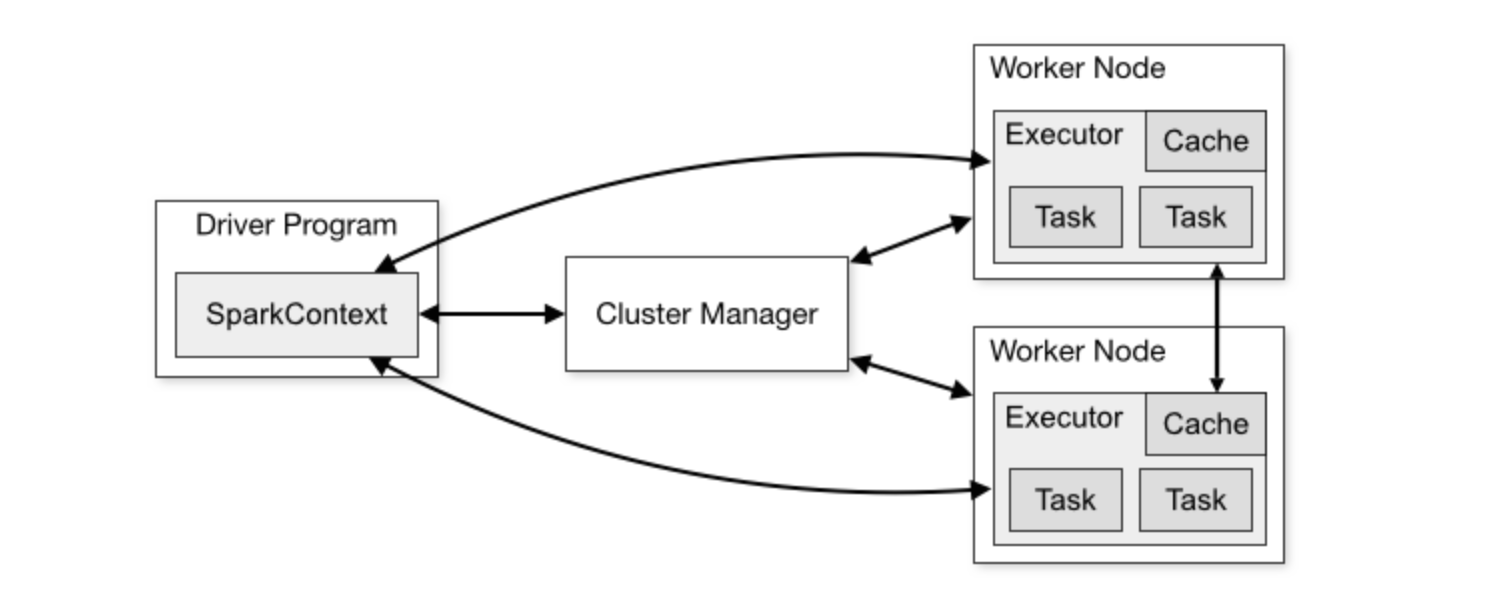
\includegraphics[width=0.6\textwidth]{chapter04/clustermanager.png}
  \bicaption[fig:4-1]{集群管理大致模式}{集群管理大致模式}{Fig}{Cluster Managing Mode}
\end{figure}

在相似轨迹获取这一应用中,根据我们的应用场景和硬件设置,我们采用\emph{Spark}自带的\emph{Standalone}集群模式,其大致设计框架如图\ref{fig:4-2}所示。

\begin{figure}[!htp]
  \centering
  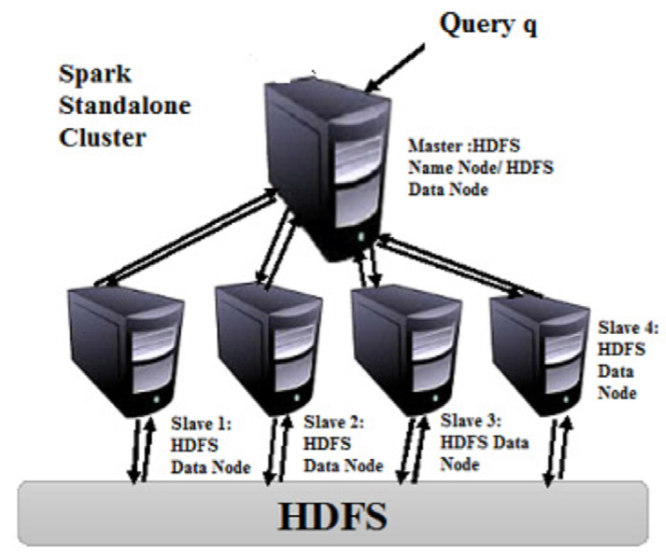
\includegraphics[width=0.5\textwidth]{chapter04/standalone.png}
  \bicaption[fig:4-2]{Spark Standalone集群结构}{Spark Standalone集群结构}{Fig}{Spark Standalone Architecture}
\end{figure}

在\emph{Standalone}集群模式中,我们通过一个在\emph{Spark}分布式环境下的简要集群管理者来简单建立集群处理环境。在这一集群环境中,主节点(\emph{Master Node})为驱动程序运行的设备节点。驱动程序不仅是与用户交互信息的接口(\emph{interface})程序,也负责分布式运行在\emph{Spark}环境中进程的运行情况。子节点们(\emph{Slave Nodes})为启动在工作节点中的进程提供运行环境,这些进程运行任务代码并在内存或磁盘中储存数据。在相似轨迹搜索中,我们将轨迹数据和预处理好的轨迹索引R树结构存储在\emph{HDFS}上,集群环境中的工作节点可以通过设定好的参数无需秘钥的共享\emph{HDFS}上已存储好的数据,这样,我们可以将相似轨迹搜索任务进一步以分布式的方法进行处理。

%\begin{figure}[!htp]
%  \centering
%  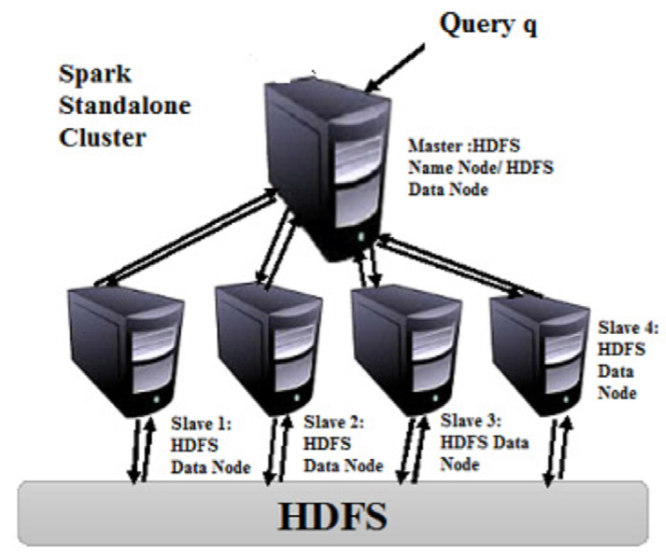
\includegraphics[width=0.5\textwidth]{chapter04/standalone.png}
%  \bicaption[fig:4-2]{这里将出现在插图索引中}{Spark Standalone集群结构}{Fig}%{Spark Standalone Architecture}
%\end{figure}


\section{分布式相似轨迹查询算法实现}
\label{sec:distributed algo}
在之前的工作描述中,我们对于相似轨迹查询的实现总会提及查询点集的数目相对较少这一前提。对于单机处理而言,如果将一整条轨迹的轨迹数据点作为输入或者查询点集过多,由于增长型k最近邻查询会对每一个查询点都进行$\lambda$-NN的搜索处理,因此整个相似轨迹的查询过程会显得相对缓慢。但有些时候,将一条轨迹作为相似轨迹查询的输入的确更简单且更人性化。在硬件设置对算法性能的约束下,借助基于地理位置点的轨迹简化方法,我们可以对前一章所涉及的相似轨迹查询方法通过加入\emph{Spark}分布式集群处理的手段,做到以一条轨迹(或数量更多的查询点)为输入的相似轨迹查询操作。具体实现思路在于,通过基于地理位置点的轨迹简化方法将一条轨迹简化为一组数量相对于单机查询要多的查询点集;然后将查询点通过分布式集群操作分配给各个子节点来进行相对于各集群节点的相似轨迹查询操作,各个子节点通过访问HDFS获取轨迹数据和轨迹R树索引;最后将结果以轨迹为关键字,以相似度为权值进行求和,选择相似度和最高的k条轨迹作为查询结果。

\subsection{基于地理位置点的轨迹简化方法}
\label{subsec:trajectory simplification based on locations}
前文描述的$Douglas$–$Peucker$轨迹简化算法主要是在保留大致形状信息的基础上对减少一些距离较近的轨迹点,从而做到轨迹简化。但对于一条轨迹而言,轨迹除了轨迹点数目这一关键字,其中一些轨迹点也具有一些隐藏的轨迹语义信息。在现实生活中,一些岔路口可能在一条轨迹中称为比较关键和重要点,或者某一个立交交通系统会成为路线中转的关键轨迹点,因此在做轨迹简化中应该尽可能地保留这些点。

在本文中,主要采用基于地理位置点的轨迹简化算法,称为$TS$ $algorithm$(TS),借鉴语义的重要性,它主要思路是从一条轨迹中查找重要的或具有特定语义的轨迹点从而进行简化和压缩。TS轨迹简化算法既保证了轨迹的大致路线也保留了重要的特定轨迹点。基于轨迹点的相似轨迹查询用户大概率会使用一些在地理意义上重要的轨迹点,因此选择基于地理语义的轨迹压缩方法能够将轨迹简化结果和相似轨迹查询匹配使用。\emph{TS}轨迹简化方法中,每个轨迹点的前进角度大小(\emph{heading direction degree})和其余相邻轨迹点之间的距离作为衡量该轨迹点权值的主要因素。通过正则化垂直距离对轨迹点权值的影响,\emph{TS}轨迹简化方法在效果上要优于$Douglas$–$Peucker$算法。

\theoremstyle{definition}
\begin{definition}
	\textbf{前进角度}(\emph{Heading direction})$h$以正北方向为基准,表示一个移动物体之后的行进方向,其中$0^\circ\leq h < 360^\circ$
\end{definition}

\theoremstyle{definition}
\begin{definition}
	\textbf{近邻前进角度改变量}(\emph{Neighbor Heading Change})$\alpha$是对于某一个轨迹点$p_i$而言,其前进角度$p_{i}.h$和之前一点$p_{i-1}$的前进角度$p_{i-1}.h$的差值,即$p_{i}.h-p_{i-1}.h$,其中其中$-180^\circ < \alpha <180^\circ$
\end{definition}

\theoremstyle{definition}
\begin{definition}
	\textbf{前进角度积累量}(\emph{Accumulated Heading Change})$\beta$表示轨迹点$p_i$前后范围$\phi$内的近邻前进角度改变量之和,即$p_{i}.\beta=\sum_{k=i-\phi}^{i+\phi}p_{k}.\alpha$。其中的$\phi$为认为预先定义好的整数阈值。
\end{definition}

\theoremstyle{definition}
\begin{definition}
	\textbf{前进量改变值}(\emph{Heading Change})$\gamma$用近邻前进角度改变量$\alpha$和前进角度积累量$\beta$定义,前进量改变值为后面两者绝对值之和,即有$p.\gamma=|p.\alpha|+|p.\beta|$
\end{definition}

\theoremstyle{definition}
\begin{definition}
	\textbf{近邻距离}(\emph{Neighbor Distance})是指一个轨迹点$p_i$到前一个轨迹点$p_{i-1}$和后一个轨迹点$p_{i+1}$(如果存在的话)的欧式距离之和,我们用符号$d$代表这一距离和,即$p_{i}.d=Dist_e(p_{i-1},p_{i})+Dist_e(p_{i},p_{i+1})$,其中,$Dist_e$在前文中已有定义,不再赘述。
\end{definition}

\theoremstyle{definition}
\begin{definition}
	\textbf{轨迹点权值}(\emph{Weight})表明轨迹点$p$的在轨迹简化中重要性大小,通过前进量改变值和近邻距离定义,即$p.\omega = p.d * p.\gamma$。
\end{definition}

根据上述定义,我们可以设计出基于地理位置点的轨迹点简化算法\ref{algo:ts}。该算法主要分为四个过程:分段、段权值排序、点权值计算和点选择。由于本工作数据集只针对车载轨迹数据,则在第一步只用进行简单的分段操作而不用进行轨迹类型分类操作。而第二步根据设定参数求出每一段的权值并通过算法定义参数保留段轨迹语义。第三步计算每个数据点的权值并通过正则化决定每一段子轨迹内选择保留相对比例的数据点。最后选择符合算法条件的点作为简化结果返回。

\begin{algorithm}
% \begin{algorithm}[H] % 强制定位
\caption{轨迹简化(Trajectory Simplification)算法}
\label{algo:ts}
\begin{algorithmic}[1] %每行显示行号
\Require 一条原始轨迹数据$Traj$, 简化后轨迹点数目$m$ % 输入
\Ensure 一条简化后只有$m$个点的轨迹$Traj'$ % 输出
\State $Traj' \gets \emptyset$
\State $Seg[] \gets Segmentation(Traj)$ //将轨迹Traj分段
\State DistributePoints(Seg[], m);	//求段权值并参数初始化
\For{Each Segment $s$ in $Seg[]$}	
	\State WeightPoints($s$)	//求点权值
    \State $s'$ $\gets$ SelectPoints($s$)	//选择点组成新的轨迹段
    \State $Traj'$ $\gets$ $Traj \cup s'$	//合并新轨迹段组成结果
  \EndFor
\end{algorithmic}
\end{algorithm}

图\ref{fig:4-3}展示了一条原始数据轨迹$Traj$通过\emph{TS}轨迹简化算法后的结果。

\begin{figure}[!htp]
  \centering
  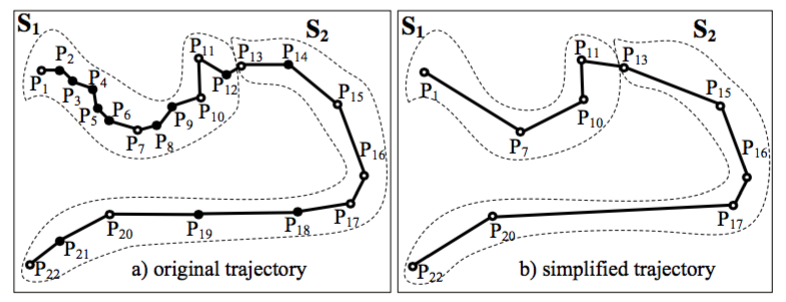
\includegraphics[width=0.5\textwidth]{chapter04/tsalgo.png}
  \bicaption[fig:4-3]{\emph{TS}算法结果样例}{\emph{TS}算法结果样例}{Fig}{An illustration of Trajectory Simplification Algorithm}
\end{figure}

\subsection{Spark分布式相似轨迹查询}
\label{subsec:distributed similar}
\emph{Spark}集群环境使得我们可以将代码分发给各个工作节点使他们处理对数据集相同的操作,这为分布式搜索相似轨迹提供了实现的基础。单机实现相似轨迹搜索为保证运行性能,给定的输入集查询点需要保证数量在某一程度上相对较小。但对于分布式处理而言,这一约束可以通过集群集计算处理予以取消。给定一条原始轨迹$Traj$,我们可以先通过基于地理位置点的轨迹简化在保留轨迹形状和轨迹中的重要位置点的同时,一定程度上减少轨迹数目。事实上,如果集群设备性能较好,我们可以略去集群计算相似轨迹前对轨迹简化这一步骤。由于本文实验设备限制,通过在集群处理前的轨迹简化能在保证结果正确性的过程中,稳定处理性能。因此,我们将轨迹简化作为集群计算前的预处理过程。

\begin{figure}[!htp]
  \centering
  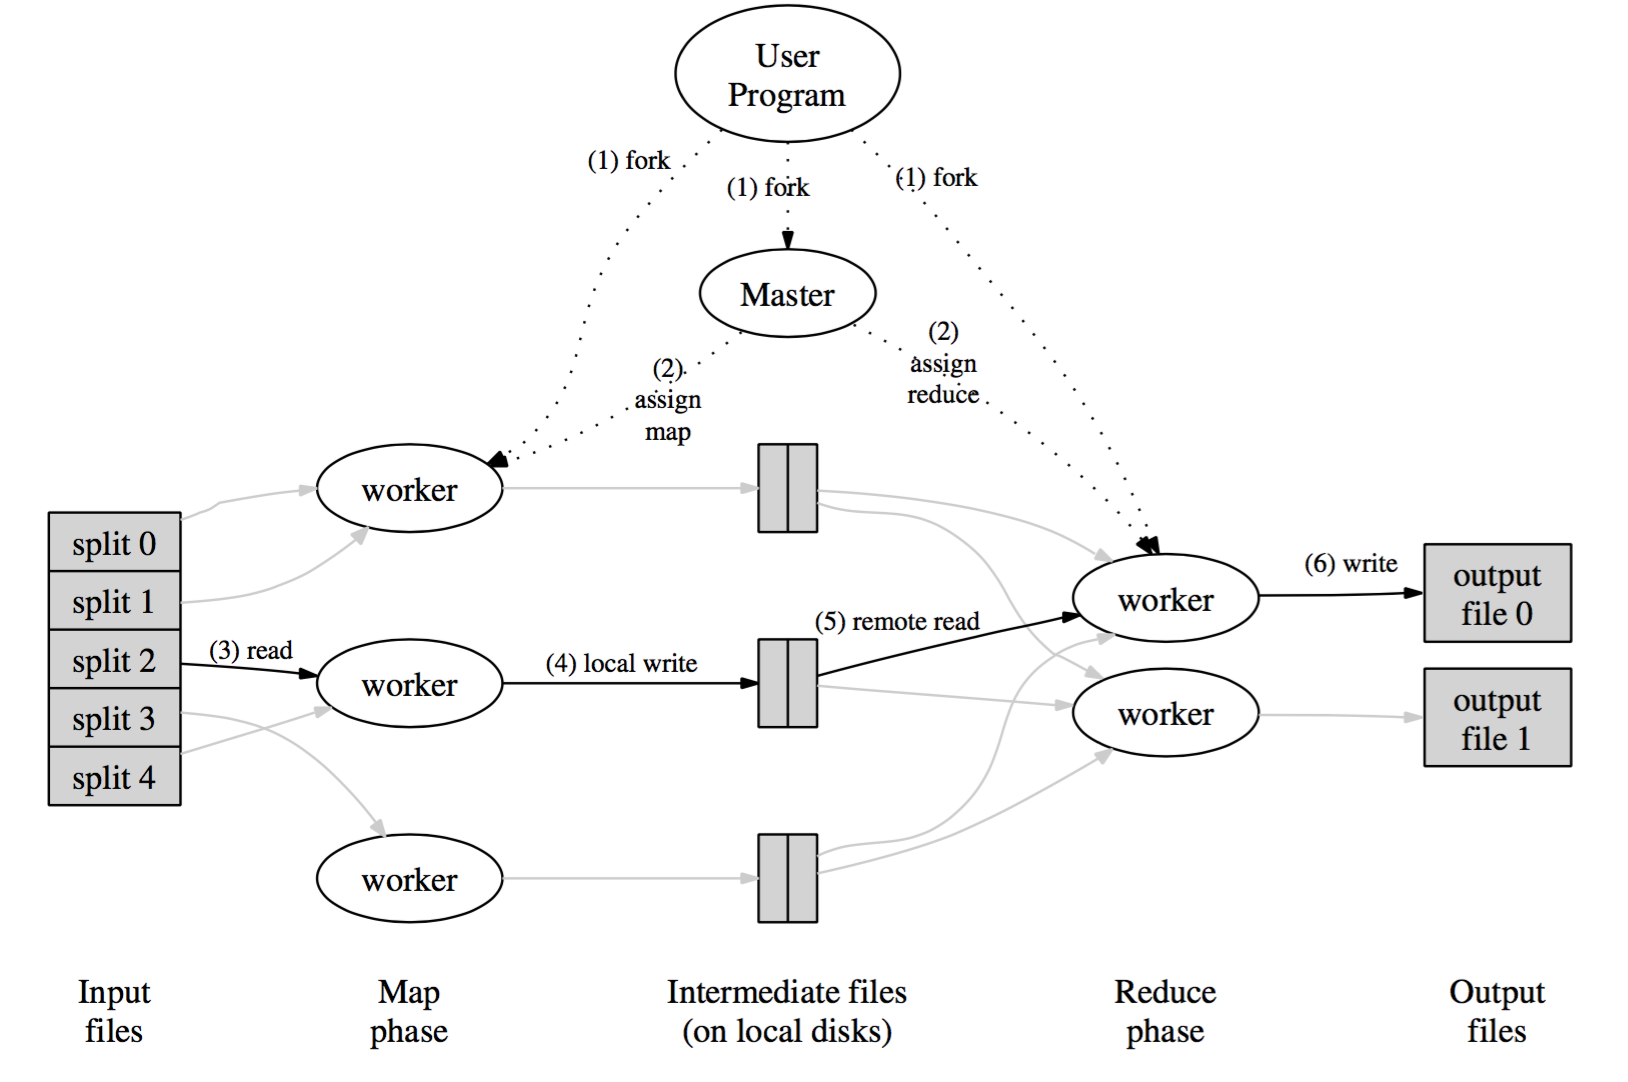
\includegraphics[width=0.85\textwidth]{chapter04/distributed.png}
  \bicaption[fig:4-4]{Spark分布式相似轨迹查询}{Spark分布式相似轨迹查询}{Fig}{Spark distributed search similar trajectories}
\end{figure}

图\ref{fig:4-4}为\emph{MapReduce}的大致处理框架,我们根据这一框架设计出分布式查询相似轨迹的大致算法。在算法中,假设我们已经完成对原始轨迹的简化得到已处理好的简化轨迹$Traj'$。首先我们通过\emph{Spark}内的\emph{partition}函数将输入数据分割,并分发给每一个工作节点(\emph{Worker Node})。对于每一个工作节点而言,他们都有了输入数据的一部分轨迹点。对于每一个工作节点而言,他们都可以将自己所拥有的部分轨迹点作为相似轨迹查询的查询点集,由于工作节点通过设置可以直接访问\emph{HDFS}上已存储的轨迹数据,我们通过主节点(\emph{Master Node})将增长型k最近邻查询代码分发给每一个工作节点并予以上运行。每个工作节点将针对各自输入查询点集所得出的k条最相似轨迹及其对应的相似度大小作为输出。通过对轨迹作为关键字合并中间查询结果,对相似度求和按相似度大小降序排列轨迹,再从中选取k条轨迹作为最终的结果。

实现细节如算法\ref{algo:distributed sim}所示。其中在运行过程中初始化\emph{Spark}运行所需的上下文变量并设置主节点信息。在\emph{map}阶段对查询点集进行查询搜索,在\emph{reduce}阶段进行关键字合并。

\begin{algorithm}
% \begin{algorithm}[H] % 强制定位
\caption{分布式相似轨迹查询算法}
\label{algo:distributed sim}
\begin{algorithmic}[1] %每行显示行号
\Require 相似轨迹查询数目$k$,一条原始轨迹数据$Traj$% 输入
\Ensure $k$条最相似轨迹$k$-$Trajs$ % 输出
\State $Traj' \gets TS(Traj)$; $\qquad$//简化轨迹
\State Initialise \emph{Spark} Context $sc$ and set Master information;
\State $RDD \gets sc.parallelize(Traj', partitionNumber)$;
\State $k$-$Trajs$ $\gets RDD.map(iknn) $ $\qquad$//工作节点分布式进行查询处理
\State $\qquad\quad.flatMap(lambda\quad x$:$x)$ $\qquad$//查询结果平铺成为一维列表或数组
\State $\qquad\quad.reduceByKey(lambda\quad x,y$:$x+y)$$\qquad$//以轨迹为关键字做相似度求和
\State $\quad\qquad.sortBy(lambda\quad x$:$x[1], descending)$$\qquad$//降序排列
\State $\quad\qquad.collect()$;
\State \textbf{return} $k$-$Trajs$; 
\end{algorithmic}
\end{algorithm}


\subsection{多请求分布式相似轨迹查询}
\label{subsec:distributed multiple}
从工业应用角度,多用户同时进行相似轨迹处理时,可以针对对多请求的分布式相似轨迹查询处理。将请求数据集根据\emph{Spark}环境默认的分割方法或自定义的分割方法,将多请求分割成多个子集,然后分配个集群中的子节点,让他们各自处理处理一部分请求。在实际生活中,作为一个交付使用的应用,在某个时段可能有多个用户请求发送给服务器端,在配置有集群环境的情况下,可以实现对请求的分布式处理,具体思路类似于上文分布式相似轨迹查询,不予以赘述。

\section{本章小结}
\label{sec:distributed-conclusion}
相似轨迹查询这一研究方法属于轨迹数据挖掘其中的分支。而随着如今GPS技术的发展和车载数据的激增,轨迹数据挖掘的数据规模通常较大,因此在处理轨迹数据过程中,单机本地操作或许无法满足轨迹挖掘的特定需求。因此,我们可以通过分布式集群处理的方法来完成大数据轨迹数据挖掘。分布式如今发展较为成熟,为我们提供了许多适应于不同应用的大数据分布式处理框架。根据\emph{MapReduce}的编程模型,我们自定义对输入、中间过程和输出的处理方法,借助分布式框架\emph{Spark}提供的接口方法能够较好的完成本文的相似轨迹查询在分布式上的实现。